\chapter{Introduzione}
\label{chap:intro}
La qui presente tesi rappresenta la terza ed ultima parte dello stage++\footnote{Lo stage++ è un progetto unico che comprende l'insieme di tre moduli: stage, project work e tesi.}, che è stato realizzato in collaborazione con il Prof. Francesco De Angelis, e-xtrategy s.r.l. e con il collega Filippo Corona.
Durante lo stage ci è stato chiesto di progettare e realizzare un’ applicazione per la visualizzazione e l' editing di modelli
3D da impiegare in ambito e-commerce.
Il prodotto che ne è risultato ha preso il nome di "CustoMyzx".

Per poter raggiungere i numerosi obettivi che questo progetto richiedeva, io e Filippo ci siamo divisi il carico di lavoro in maniera il più possibile equa: una metà del progetto si è focalizzata sul front end, e quindi sull’interfaccia mirata all’utente, l’altra invece sul back end, estraneo a quest’ultimo.
Nella prima fase della progettazione, i due semi-progetti sono stati nominati rispettivamente “unicam-product-viewer” e “unicam-product-editor” ai fini di una distinzione tra questi.
Io mi sono occupato della parte back end, e quindi di "unicam-product-editor", mentre Filippo, in modo complementare, ha sviluppato la parte front end e il relativo sotto-progetto:"unicam-product-viewer".

Quindi il progetto è composto dalle seguenti parti:
\begin{enumerate}
	\item Il back end
	\item Una web app come interfaccia per il back end
	\item Il front end
	\item Il configuratore 3D e in realtà aumentata sviluppato tramite web app
\end{enumerate}
Tutte le parti di CustoMyzx sono state scritte in Javascript ad eccezione di uno script esterno realizzato in Python.

Questa tesi tratterà nella fattispecie i primi due punti: la realizzazione dell' applicazione web mediante l'utilizzo del MEAN Stack\index{MEAN} piuttosto che il tradizionale LAMP Stack\footnote{Acronimo (Linux, Apache, MySQL, PHP) che indica una piattaforma software per lo sviluppo di applicazioni web}, e l' uso del modello architetturale nelle web app chiamato "Long Polling".

Il codice completo del progetto è disponibile nei due repository
\begin{enumerate}
	\item \url{www.github.com/e-xtrategy/unicam-product-editor}
	\item \url{www.github.com/e-xtrategy/unicam-product-viewer}
\end{enumerate} 

\section{Progettazione}
La fase di progettazione si è sviluppata secondo il metodo extrategy: l'azienda basa lo sviluppo di software sulle metodologie agili, più adatte ad ambienti dinamici come lo è il web, come ad esempio la formazione di team di sviluppo piccoli, cross-funzionali e auto-organizzati, 
lo sviluppo iterativo e incrementale, la pianificazione adattiva, e il coinvolgimento diretto e continuo del cliente nel processo di sviluppo.

In particolare, abbiamo utilizzato una via di mezzo tra Scrum e Kanban.

L'utilizzo del framework Scrum\cite{scrum}\index{Scrum} consiste nel passaggio attraverso una serie di iterazioni a intervalli di tempo regolari, dette sprint\index{Sprint}, che consentono di consegnare il progetto passo dopo passo al cliente e con cadenza costante. Attraverso la giusta frequenza adottata per gli sprint, si è capaci di fare delle stime più corrette, e inoltre si possono ricevere feedback in tempo reale sul lavoro svolto.
Ogni sprint si divide in quattro fasi:
\begin{enumerate}
	\item \textbf{Pianificazione}: incontro iniziale in cui si definisce cosa fare con lo sprint corrente.
	\item \textbf{Scrum giornaliero}: mini incontro giornaliero della durata di una decina di minuti per sincronizzare il team. 
	\item \textbf{Demo}: incontro per illustrare il lavoro svolto dal team.
	\item \textbf{Retrospettiva}: una revisione di ciò che è stato fatto, esponendo anche i possibili miglioramenti attuabili.
\end{enumerate} 

Il Kanban\cite{kanban}\index{kanban} serve per tenere d'occhio l'avanzamento dei lavori durante gli sprint; la kanban board dunque non è altro che una lavagna atta a visualizzare e ottimizzare il flusso di lavoro del team. Un classico kanban può essere dato da una lavagna o da un' intera parete (es. e-xtrategy), ma per il nostro sviluppo software abbiamo utilizzato una board virtuale, in cui abbiamo riscontrato aspetti positivi quali tracciabilità, facilità di collaborazione, accessibilità delocalizzata.

Le funzioni di una kanban sono comunque quelle di standardizzare il flusso di lavoro e di assicurare una buona visibilità e visualizzazione del lavoro del team, per poter individuare e risolvere tempestivamente eventuali criticità.
Questa metodologia inoltre è basata sulla trasparenza e sulla comunicazione, pertanto la kanban board dovrebbe essere vista come una visione oggettiva e veritiera agli occhi del team.
Di norma si prevedono tre step: To Do, In Progress e Done, che noi abbiamo rinominato rispettivamente in Backlog, Sprint e Approved.

Con questa impostazione, Antonio Dell'Ava, il nostro tutor in e-xtrategy, ci ha guidato verso lo strumento più utile per tenere traccia dello sviluppo del software, implementare le user-stories e coordinare gli sviluppatori assegnati al progetto, in questo caso io e Filippo: Trello ci ha permesso di gestire il nostro piccolo team senza applicare alla lettera Kanban, ma tramite una semplice todo list.

Trello\index{Trello}\cite{trello} è un gestore di progetti basato sul web e realizzato da Fog Creek Software nel 2011.
Qui il progetto è rappresentato da schede, a loro volta contenenti liste corrispondenti ad elenchi di attività. Le liste sono formate da card, che rappresentano le singole attività.
Queste card si possono spostare tra le diverse liste con il metodo drag and drop, per seguire il normale flusso di sviluppo passando dalla lista "da fare" ad esempio alla lista "fatto" una volta che è stata realizzata questa parte del progetto.

Nel nostro caso ogni card rappresenta una user-story, ossia una funzionalità utile al raggiungimento di un obiettivo di business, una descrizione volutamente generica di una caratteristica che il software deve avere, e che può essere stata esplicitamente richiesta dal cliente, essere necessità o consiglio dello sviluppatore, o essere nata dalla discussione tra i due soggetti.
Ogni card può vedersi assegnata ad uno o più sviluppatori, e queste si possono organizzare, insieme alle loro schede, in raggruppamenti personalizzati.
Si possono inserire inoltre commenti, allegati, date di scadenza, voti e liste di controllo in ogni card.
Nel complesso, la suddivisione di un progetto in schede/liste, che a loro volta sono suddivise in card, formano un insieme di dati su misura organizzati in modo gerarchico, che rende più facile ed efficace la gestione dei progetti, ma di conseguenza anche le attività di tutta l' organizzazione.

\begin{figure}[h]
	\centering
	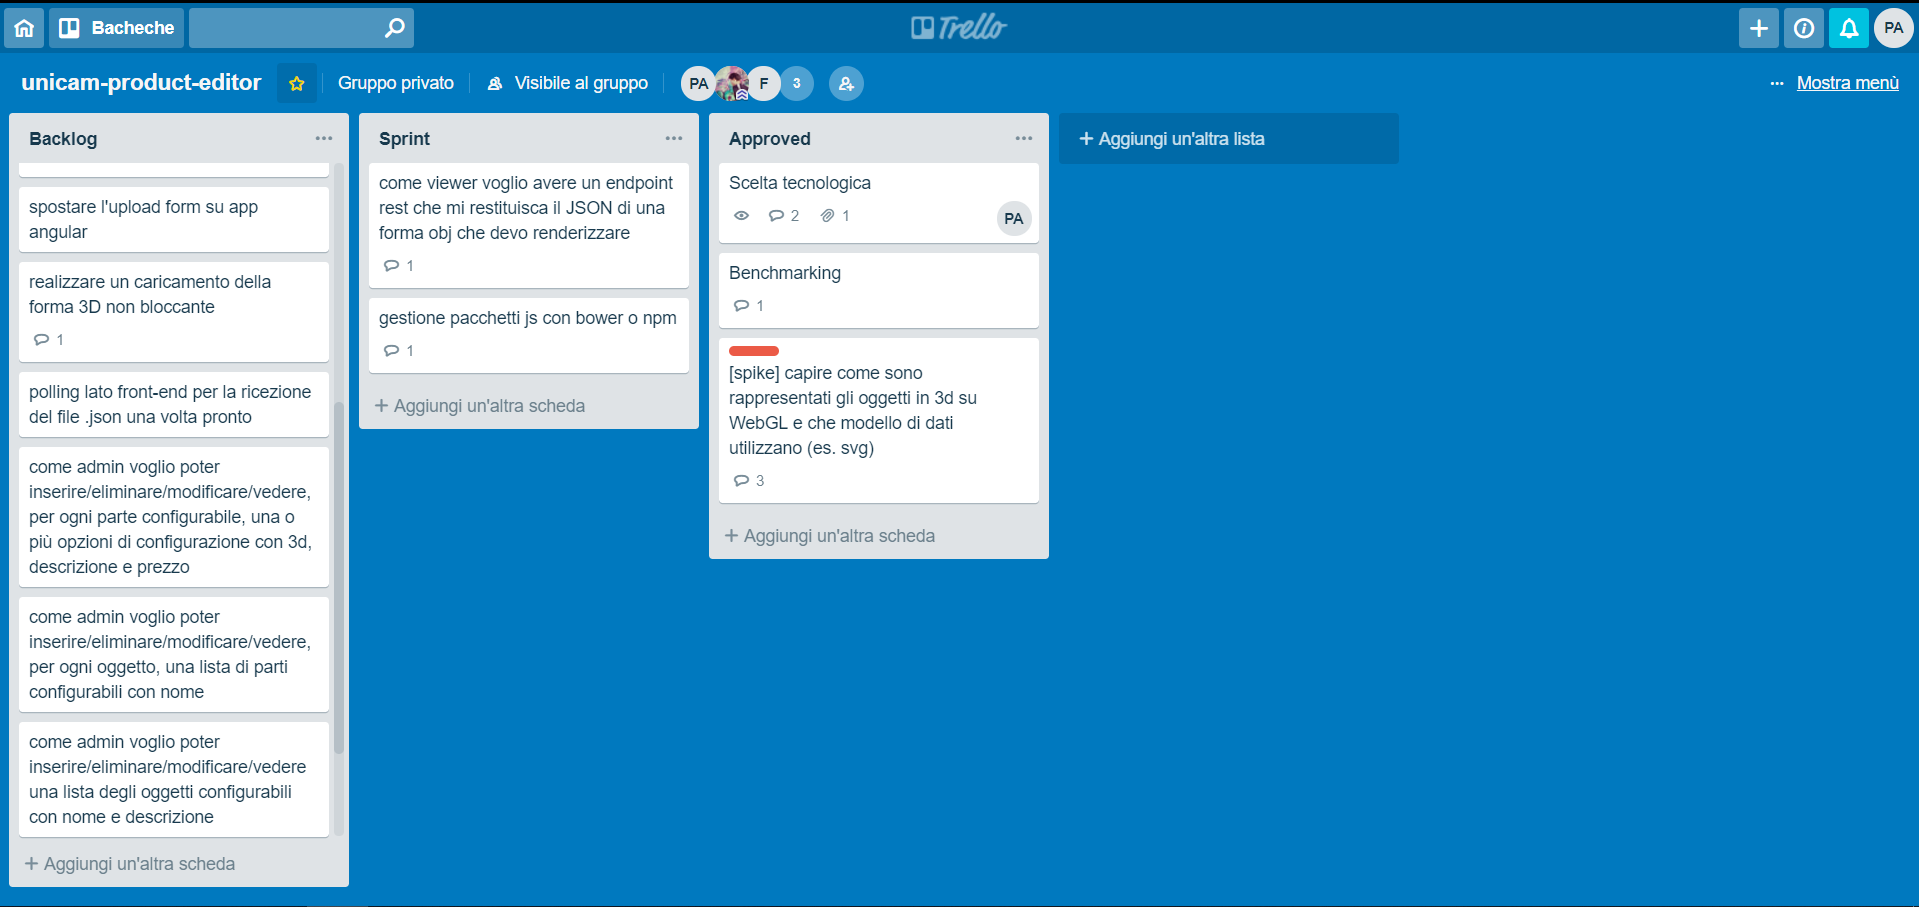
\includegraphics[scale=0.35]{Immagini/trello_start.png} 
	\caption{Organizzazione di unicam-product-editor su Trello}
\end{figure}

\section{Analisi}
Si vuole realizzare una applicazione web che permetta di gestire gli oggetti 3D tramite upload, modifica e visualizzazione in formato .JSON.
Il backend deve ricevere in input una forma 3D sotto forma di file in formato .obj, convertirlo in .JSON e fornire i servizi REST\index{REST}.
Un utente deve poter inserire l'oggetto 3D tramite l'uploader, modificare i metadati dell'oggetto convertito e visualizzare il file convertito attraverso un apposito endpoint una volta effettuata l'autenticazione.
Il processo di upload e conversione in particolare non deve essere bloccante, in quanto l'utente deve poter continuare ad utilizzare il servizio anche durante l'upload di una forma 3D molto grande.

La struttura dei documenti all'interno del progetto sarà la seguente:
\begin{itemize}
	\item[$\bullet$] Lista
	\begin{itemize}
		\item[$\bullet$] Oggetto
		\item[$\cdot$] Omino Lego
		\begin{itemize}
			\item[$\bullet$] Parte
			\item[$\cdot$] Testa
			\item[$\cdot$] Busto
			\begin{itemize}
				\item[$\bullet$] Opzione
				\item[$\cdot$] Busto standard
				\item[$\cdot$] Busto con papillon
				\item[$\cdot$] Busto con cravatta
			\end{itemize}
		\end{itemize}
	\end{itemize}
\end{itemize}

Le user stories derivanti da questo processo di analisi sono le seguenti:

\begin{longtable}{|c|l|}
	% intestazione iniziale
	\hline
	\multicolumn{1}{|c|}{\textbf{Numero}} & \multicolumn{1}{c|}{\textbf{Descrizione}} \\
	\endfirsthead
	% intestazione normale
	\multicolumn{2}{l}{\footnotesize\itshape\tablename~\thetable:
		continua dalla pagina precedente} \\
	\hline
	\multicolumn{1}{|c|}{\textbf{Numero}} & \multicolumn{1}{c|}{\textbf{Descrizione}} \\
	\endhead
	% piede normale
	\multicolumn{2}{r}{\footnotesize\itshape\tablename~\thetable:
		continua nella prossima pagina} \\
	\endfoot
	% piede finale
	\multicolumn{2}{r}{} \\
	\endlastfoot
	\hline
	01 & Scelta tecnologica.\\
	\hline
	02 & Benchmarking.\\
	\hline
	03 & Capire come sono rappresentati gli oggetti in 3d su WebGL e che\\ 
	& modello di dati utilizzano (es. svg).\\
	\hline
	04 & Come admin voglio poter inserire/eliminare/modificare/vedere una\\
	& lista degli oggetti configurabili con nome e descrizione.\\
	\hline
	05 & Come admin voglio poter inserire/eliminare/modificare/vedere,\\  & per ogni oggetto, una lista di parti configurabili con nome.\\
	\hline
	06 & Come admin voglio poter inserire/eliminare/modificare/vedere,\\  & per ogni parte configurabile, una o più opzioni di configurazione\\ & con 3D, descrizione e prezzo.\\
	\hline
	07 & Come viewer voglio avere un endpoint rest che mi restituisca\\   & il JSON di una forma obj che devo renderizzare.\\
	\hline
	08 & Creare app single-page con Angular.\\
	\hline
	09 & Realizzare un caricamento della forma 3D non bloccante\\ & (upload, conversione ed endpoint in modo sincrono).\\
	\hline
	10 & Polling lato front-end per la ricezione del file .JSON una volta pronto.\\
	\hline
	\caption{User stories}
	\label{tab:user:sto} \\
\end{longtable} 

Il diagramma di Gantt riguardante l'assegnazione dei task e lo svolgimento temporale, è il seguente:
\begin{figure}[h]
	\centering
	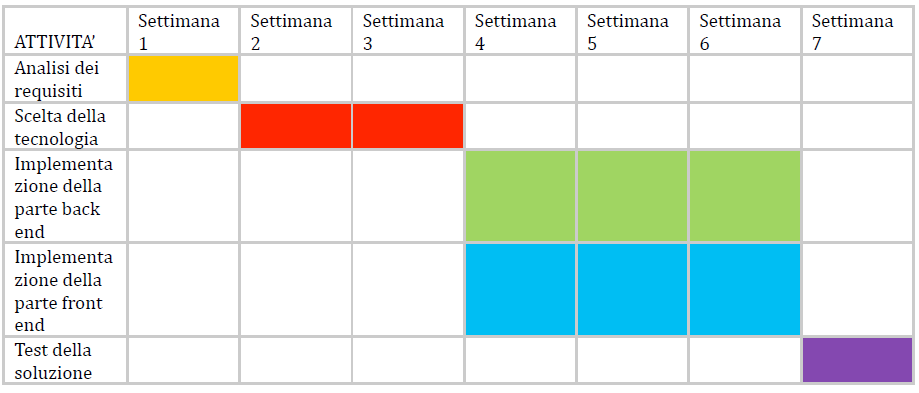
\includegraphics[scale=0.7]{Immagini/piano_realizzazione_progetto.png}
	\caption{Piano di realizzazione del progetto}
\end{figure}